\documentclass[11pt,a4paper]{report}
\usepackage[textwidth=37em,vmargin=30mm]{geometry}
\usepackage{calc,xunicode,amsmath,amssymb,paralist,enumitem,tabu,booktabs,datetime2,xeCJK,xeCJKfntef,listings}
\usepackage{tocloft,fancyhdr,tcolorbox,xcolor,graphicx,eso-pic,xltxtra,xelatexemoji}

\newcommand{\envyear}[0]{2025}
\newcommand{\envdatestr}[0]{2025-04-20}
\newcommand{\envfinaldir}[0]{webdb/2025/20250420/final}

\usepackage[hidelinks]{hyperref}
\hypersetup{
    colorlinks=false,
    pdfpagemode=FullScreen,
    pdftitle={Web Digest - \envdatestr}
}

\setlength{\cftbeforechapskip}{10pt}
\renewcommand{\cftchapfont}{\rmfamily\bfseries\large\raggedright}
\setlength{\cftbeforesecskip}{2pt}
\renewcommand{\cftsecfont}{\sffamily\small\raggedright}

\setdefaultleftmargin{2em}{2em}{1em}{1em}{1em}{1em}

\usepackage{xeCJK,xeCJKfntef}
\xeCJKsetup{PunctStyle=plain,RubberPunctSkip=false,CJKglue=\strut\hskip 0pt plus 0.1em minus 0.05em,CJKecglue=\strut\hskip 0.22em plus 0.2em}
\XeTeXlinebreaklocale "zh"
\XeTeXlinebreakskip = 0pt


\setmainfont{Brygada 1918}
\setromanfont{Brygada 1918}
\setsansfont{IBM Plex Sans}
\setmonofont{JetBrains Mono NL}
\setCJKmainfont{Noto Serif CJK SC}
\setCJKromanfont{Noto Serif CJK SC}
\setCJKsansfont{Noto Sans CJK SC}
\setCJKmonofont{Noto Sans CJK SC}

\setlength{\parindent}{0pt}
\setlength{\parskip}{8pt}
\linespread{1.15}

\lstset{
	basicstyle=\ttfamily\footnotesize,
	numbersep=5pt,
	backgroundcolor=\color{black!5},
	showspaces=false,
	showstringspaces=false,
	showtabs=false,
	tabsize=2,
	captionpos=b,
	breaklines=true,
	breakatwhitespace=true,
	breakautoindent=true,
	linewidth=\textwidth
}






\newcommand{\coverpic}[2]{
    % argv: itemurl, authorname
    Cover photo by #2~~(\href{#1}{#1})
}
\newcommand{\makeheader}[0]{
    \begin{titlepage}
        % \newgeometry{hmargin=15mm,tmargin=21mm,bmargin=12mm}
        \begin{center}
            
            \rmfamily\scshape
            \fontspec{BaskervilleF}
            \fontspec{Old Standard}
            \fontsize{59pt}{70pt}\selectfont
            WEB\hfill DIGEST
            
            \vfill
            % \vskip 30pt
            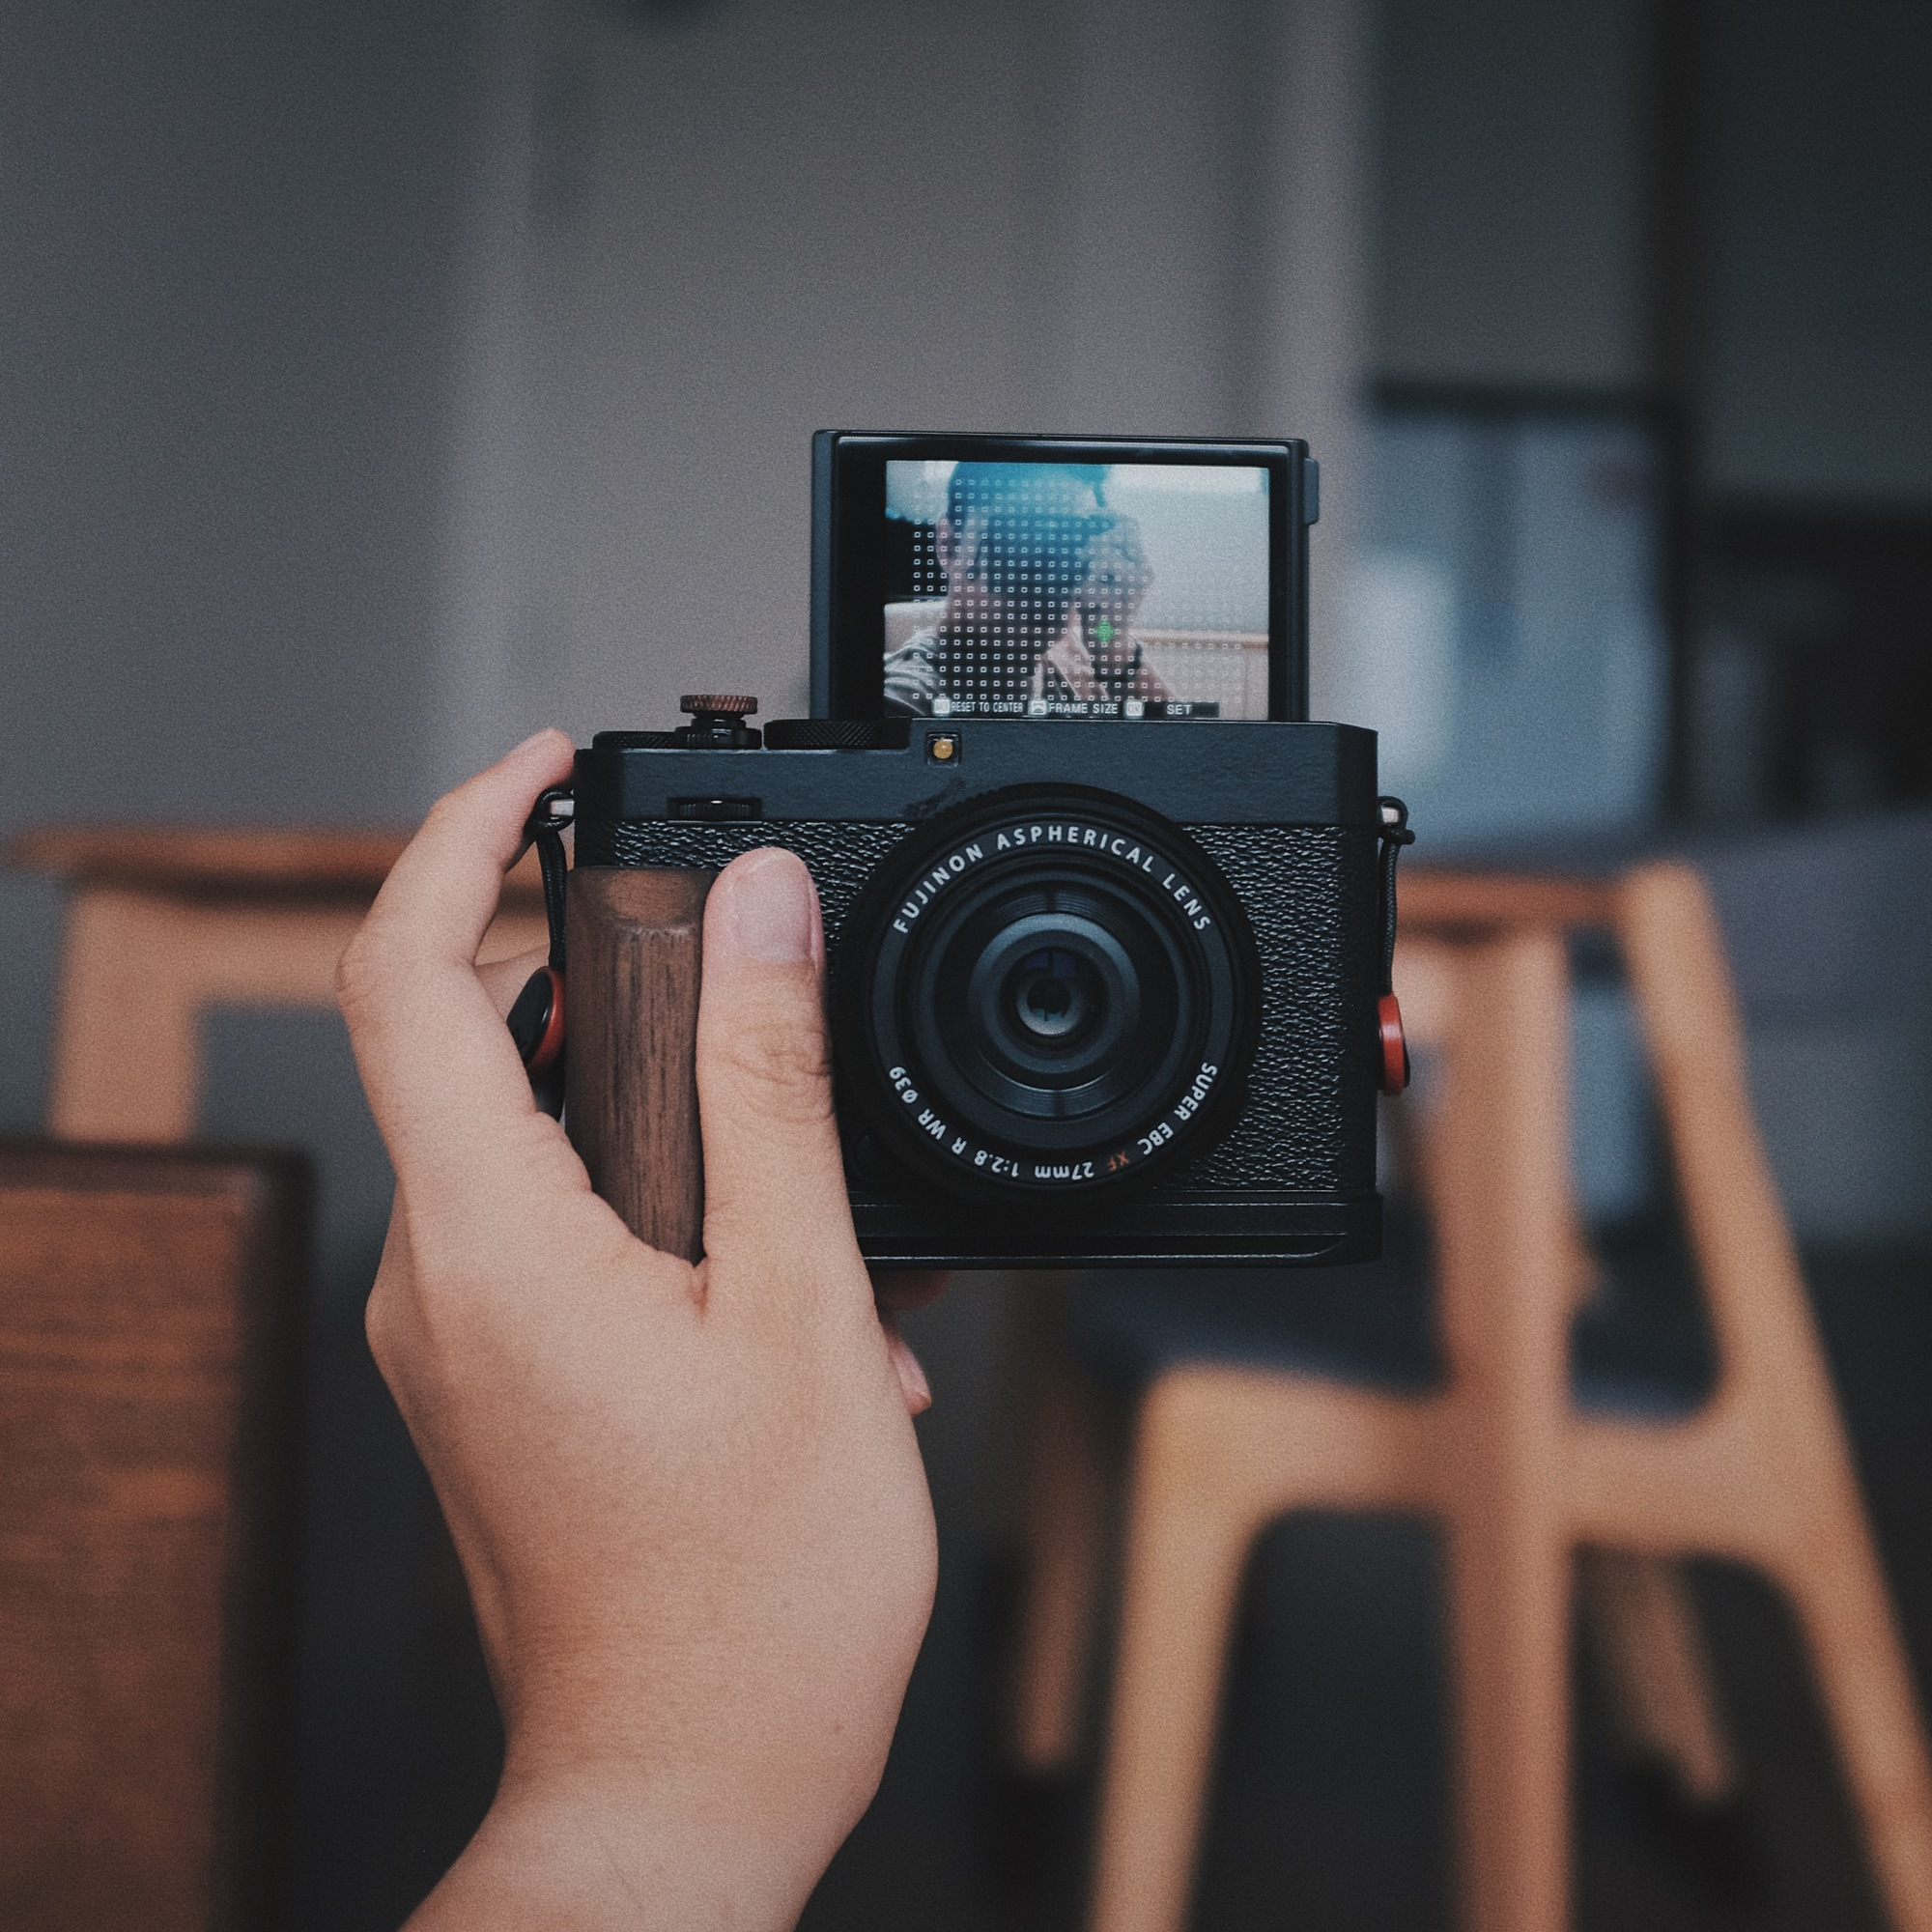
\includegraphics[width=\linewidth]{\envfinaldir/coverpic-prod.jpg}\par
            % \vskip 30pt
            \vfill

            \normalsize\rmfamily\scshape
            \copyright{} The Web Digest Project \hfill\large \envdatestr
        \end{center}
    \end{titlepage}
    % \restoregeometry
}
\newcommand{\simplehref}[1]{%
    \textcolor{blue!80!green}{\href{#1}{#1}}%
}
\renewcommand{\contentsname}{\center\Huge\sffamily\bfseries Contents\par\vskip 20pt}
\newcounter{ipartcounter}
\setcounter{ipartcounter}{0}
\newcommand{\ipart}[1]{
    % \vskip 20pt
    \clearpage
    \stepcounter{ipartcounter}
    \phantomsection
    \addcontentsline{toc}{chapter}{#1}
    % \begin{center}
    %     \Huge
    %     \sffamily\bfseries
    %     #1
    % \end{center}
    % \vskip 20pt plus 7pt
}
\newcounter{ichaptercounter}
\setcounter{ichaptercounter}{0}
\newcommand{\ichapter}[1]{
    % \vskip 20pt
    \clearpage
    \stepcounter{ichaptercounter}
    \phantomsection
    \addcontentsline{toc}{section}{\numberline{\arabic{ichaptercounter}}#1}
    \begin{center}
        \Huge
        \sffamily\bfseries
        #1
    \end{center}
    \vskip 20pt plus 7pt
}
\newcommand{\entrytitlefont}[1]{\subsection*{\raggedright\Large\sffamily\bfseries#1}}
\newcommand{\entryitemGeneric}[2]{
    % argv: title, url
    \parbox{\linewidth}{
        \entrytitlefont{#1}\par\vskip 5pt
        \footnotesize\ttfamily\mdseries
        \simplehref{#2}
    }\vskip 11pt plus 11pt minus 1pt
}
\newcommand{\entryitemGithub}[3]{
    % argv: title, url, desc
    \parbox{\linewidth}{
        \entrytitlefont{#1}\par\vskip 5pt
        \footnotesize\ttfamily\mdseries
        \simplehref{#2}\par\vskip 5pt
        \small\rmfamily\mdseries#3
    }\vskip 11pt plus 11pt minus 1pt
}
\newcommand{\entryitemAp}[3]{
    % argv: title, url, desc
    \parbox{\linewidth}{
        \entrytitlefont{#1}\par\vskip 5pt
        \footnotesize\ttfamily\mdseries
        \simplehref{#2}\par\vskip 5pt
        \small\rmfamily\mdseries#3
    }\vskip 11pt plus 11pt minus 1pt
}
\newcommand{\entryitemHackernews}[3]{
    % argv: title, hnurl, rawurl
    % \parbox{\linewidth}{
    %     \entrytitlefont{#1}\par\vskip 5pt
    %     \footnotesize\ttfamily\mdseries
    %     \simplehref{#3}\par
    %     \textcolor{black!50}{\href{#2}{#2}}
    % }\vskip 11pt plus 11pt minus 1pt
    \begin{minipage}{\linewidth}
            \entrytitlefont{#1}\par\vskip 5pt
            \footnotesize\ttfamily\mdseries
            \simplehref{#3}\par
            \textcolor{black!50}{\href{#2}{#2}}
    \end{minipage}\par\vskip 11pt plus 11pt minus 1pt
}







\begin{document}

\makeheader

\tableofcontents\clearpage




\ipart{Developers}
\ichapter{Hacker News}
\entryitemTwoLinks{Vibe Coding is not an excuse for low-quality work}{https://news.ycombinator.com/item?id=43739037}{https://addyo.substack.com/p/vibe-coding-is-not-an-excuse-for}

\entryitemTwoLinks{The Web Is Broken – Botnet Part 2}{https://news.ycombinator.com/item?id=43738603}{https://jan.wildeboer.net/2025/04/Web-is-Broken-Botnet-Part-2/}

\entryitemTwoLinks{Raspberry Pi Lidar Scanner}{https://news.ycombinator.com/item?id=43738561}{https://github.com/PiLiDAR/PiLiDAR}

\entryitemTwoLinks{Ssl.com: DCV bypass and issue fake certificates for any MX hostname}{https://news.ycombinator.com/item?id=43738485}{https://bugzilla.mozilla.org/show\_bug.cgi?id=1961406}

\entryitemTwoLinks{Librarians are dangerous}{https://news.ycombinator.com/item?id=43736791}{https://bradmontague.substack.com/p/librarians-are-dangerous}

\entryitemTwoLinks{Packing Input Frame Context in Next-Frame Prediction Models for Video Generation}{https://news.ycombinator.com/item?id=43736193}{https://lllyasviel.github.io/frame\_pack\_gitpage/}

\entryitemTwoLinks{Android phones will soon reboot themselves after sitting unused for three days}{https://news.ycombinator.com/item?id=43735902}{https://arstechnica.com/gadgets/2025/04/android-phones-will-soon-reboot-themselves-after-sitting-unused-for-3-days/}

\entryitemTwoLinks{Claude Code: Best practices for agentic coding}{https://news.ycombinator.com/item?id=43735550}{https://www.anthropic.com/engineering/claude-code-best-practices}

\entryitemTwoLinks{Restoring the Galaxian3 Theatre 6, 1992 six player arcade machine}{https://news.ycombinator.com/item?id=43735239}{https://philwip.com/2025/04/14/galaxian-3-project-revival/}

\entryitemTwoLinks{A Map of British Dialects (2023)}{https://news.ycombinator.com/item?id=43734953}{https://starkeycomics.com/2023/11/07/map-of-british-english-dialects/}

\entryitemTwoLinks{Show HN: Undercutf1 – F1 Live Timing TUI with Driver Tracker, Variable Delay}{https://news.ycombinator.com/item?id=43734910}{https://github.com/JustAman62/undercut-f1}

\entryitemTwoLinks{Show HN: Goldbach Conjecture up to 4*10^18+7*10^13}{https://news.ycombinator.com/item?id=43734583}{https://medium.com/@jay\_gridbach/grid-computing-shatters-world-record-for-goldbach-conjecture-verification-1ef3dc58a38d}

\entryitemTwoLinks{JavaScript Views, the Hard Way – A Pattern for Writing UI}{https://news.ycombinator.com/item?id=43733636}{https://github.com/matthewp/views-the-hard-way}

\entryitemTwoLinks{Hands-On Large Language Models}{https://news.ycombinator.com/item?id=43733553}{https://github.com/HandsOnLLM/Hands-On-Large-Language-Models}

\entryitemTwoLinks{Cozy video games can quell stress and anxiety}{https://news.ycombinator.com/item?id=43733097}{https://www.reuters.com/business/retail-consumer/cozy-video-games-can-quell-stress-anxiety-2025-01-27/}

\entryitemTwoLinks{Hypertext TV}{https://news.ycombinator.com/item?id=43732805}{https://hypertext.tv/}

\entryitemTwoLinks{OpenAI's new reasoning AI models hallucinate more}{https://news.ycombinator.com/item?id=43732506}{https://techcrunch.com/2025/04/18/openais-new-reasoning-ai-models-hallucinate-more/}

\entryitemTwoLinks{I passionately hate hype, especially the AI hype}{https://news.ycombinator.com/item?id=43732047}{https://unixdigest.com/articles/i-passionately-hate-hype-especially-the-ai-hype.html}

\entryitemTwoLinks{Full Text Search of US Court records}{https://news.ycombinator.com/item?id=43731552}{https://www.judyrecords.com/}

\entryitemTwoLinks{UML diagram for the DDD example in Evans' book}{https://news.ycombinator.com/item?id=43731250}{https://github.com/takaakit/uml-diagram-for-ddd-example-in-evans-book}\ichapter{Phoronix}
\entryitemGeneric{\hskip 0pt{}Intel Simplifies Its Firmware License For The Integrated Sensor Hub "ISH"}{https://www.phoronix.com/news/Intel-ISH-Simplified-Firmware}

\entryitemGeneric{\hskip 0pt{}FFmpeg AV1 Vulkan Encoder Patch Posted}{https://www.phoronix.com/news/FFmpeg-AV1-Vulkan-Encoder}

\entryitemGeneric{\hskip 0pt{}GCC 16 Adding Support For GNU/Hurd On RISC-V Targets}{https://www.phoronix.com/news/GCC-16-RISC-V-GNU-Hurd-Targets}

\entryitemGeneric{\hskip 0pt{}Google Engineers Exploring Distributed ThinLTO Builds Of The Linux Kernel}{https://www.phoronix.com/news/Distributed-ThinkLTO-Linux-Kern}

\entryitemGeneric{\hskip 0pt{}KDE Preps More Wayland Improvements, Addresses Another Possible KWin Crash}{https://www.phoronix.com/news/KDE-Plasma-Mid-April-2025}

\entryitemGeneric{\hskip 0pt{}Linux 6.15-rc3 To Bring AMD Zen 5 Microcode Protection, Intel Bartlett Lake ID Addition}{https://www.phoronix.com/news/Linux-6.15-rc3-x86-Fixes}

\entryitemGeneric{\hskip 0pt{}Slightly Faster AES-XTS Performance For AVX-512 CPUs Expected With Linux 6.16}{https://www.phoronix.com/news/Linux-6.16-AES-XTS-AVX-512-Fast}

\entryitemGeneric{\hskip 0pt{}Initial Linux Gaming/Graphics Performance For The NVIDIA GeForce RTX 5060 Ti}{https://www.phoronix.com/review/nvidia-rtx-5060ti-linux-gaming}

\entryitemGeneric{\hskip 0pt{}Intel Xe Driver Adds Fan Speed Reporting For Linux 6.16, BMG Instability Being Debugged}{https://www.phoronix.com/news/Intel-Xe-Linux-6.16-Fan-Speeds}\ichapter{Dribbble}
\entryitemGeneric{\hskip 0pt{}Tanuki - Raccoon, Animal Logo Design}{https://dribbble.com/shots/25917338-Tanuki-Raccoon-Animal-Logo-Design}

\entryitemGeneric{\hskip 0pt{}Case study: Educational Website on Space Pollution}{https://dribbble.com/shots/25914349-Case-study-Educational-Website-on-Space-Pollution}

\entryitemGeneric{\hskip 0pt{}Columbus Rapids®}{https://dribbble.com/shots/25915181-Columbus-Rapids}

\entryitemGeneric{\hskip 0pt{}UNIC // Mobile App}{https://dribbble.com/shots/25913185-UNIC-Mobile-App}

\entryitemGeneric{\hskip 0pt{}Phantom concept with Widget}{https://dribbble.com/shots/25911511-Phantom-concept-with-Widget}

\entryitemGeneric{\hskip 0pt{}Cute Easter Bunny Mascot}{https://dribbble.com/shots/25914543-Cute-Easter-Bunny-Mascot}

\entryitemGeneric{\hskip 0pt{}Crypto Widget}{https://dribbble.com/shots/25913330-Crypto-Widget}

\entryitemGeneric{\hskip 0pt{}Startup Branding for Holidu: visual identity, brand design}{https://dribbble.com/shots/25903662-Startup-Branding-for-Holidu-visual-identity-brand-design}

\entryitemGeneric{\hskip 0pt{}Mountains to Sea}{https://dribbble.com/shots/25910072-Mountains-to-Sea}

\entryitemGeneric{\hskip 0pt{}Forg Logo}{https://dribbble.com/shots/25910287-Forg-Logo}

\entryitemGeneric{\hskip 0pt{}Cute Unicorn Mascot}{https://dribbble.com/shots/25909768-Cute-Unicorn-Mascot}

\entryitemGeneric{\hskip 0pt{}Logolounge Book 15 Entry - Client Work}{https://dribbble.com/shots/25909344-Logolounge-Book-15-Entry-Client-Work}

\entryitemGeneric{\hskip 0pt{}Reindeer in Golden Light 🦌}{https://dribbble.com/shots/25905633-Reindeer-in-Golden-Light}

\entryitemGeneric{\hskip 0pt{}Altitude}{https://dribbble.com/shots/25902364-Altitude}

\entryitemGeneric{\hskip 0pt{}Logo Collection > Birds Volume 03}{https://dribbble.com/shots/25905911-Logo-Collection-Birds-Volume-03}

\entryitemGeneric{\hskip 0pt{}Automation builder - Wireframes}{https://dribbble.com/shots/25904187-Automation-builder-Wireframes}

\entryitemGeneric{\hskip 0pt{}Details - Amplemarket Logo \& Visual Identity}{https://dribbble.com/shots/25904732-Details-Amplemarket-Logo-Visual-Identity}

\entryitemGeneric{\hskip 0pt{}LogoLounge Book 15 Entry}{https://dribbble.com/shots/25904019-LogoLounge-Book-15-Entry}

\entryitemGeneric{\hskip 0pt{}FarmGirl Fresh®}{https://dribbble.com/shots/25905838-FarmGirl-Fresh}

\entryitemGeneric{\hskip 0pt{}Road Tripping}{https://dribbble.com/shots/25900418-Road-Tripping}

\entryitemGeneric{\hskip 0pt{}Lion sketches}{https://dribbble.com/shots/25898381-Lion-sketches}

\entryitemGeneric{\hskip 0pt{}Bloksy Logo Design - City, Colorful, Building, Construction}{https://dribbble.com/shots/25898764-Bloksy-Logo-Design-City-Colorful-Building-Construction}

\entryitemGeneric{\hskip 0pt{}Cute Shiba Catching a Ball}{https://dribbble.com/shots/25900210-Cute-Shiba-Catching-a-Ball}

\entryitemGeneric{\hskip 0pt{}Corti: Visual identity exploration}{https://dribbble.com/shots/25899331-Corti-Visual-identity-exploration}


\ipart{Developers~~~~(zh-Hans)}
\ichapter{Solidot}
\entryitemGeneric{\hskip 0pt{}机器人在首届人机半程马拉松比赛中惨败给人类}{https://www.solidot.org/story?sid=81091}

\entryitemGeneric{\hskip 0pt{}气候变化会增加大米的砷含量}{https://www.solidot.org/story?sid=81090}

\entryitemGeneric{\hskip 0pt{}研究称成年人食用植物性蛋白质有助于长寿}{https://www.solidot.org/story?sid=81089}

\entryitemGeneric{\hskip 0pt{}全球多达 17\% 的农田受到重金属污染 }{https://www.solidot.org/story?sid=81088}

\entryitemGeneric{\hskip 0pt{}好奇号在火星上发现碳酸盐}{https://www.solidot.org/story?sid=81087}

\entryitemGeneric{\hskip 0pt{}Microsoft 365 默认禁用 ActiveX}{https://www.solidot.org/story?sid=81086}

\entryitemGeneric{\hskip 0pt{}日本科学家用培养基生长出整块鸡肉}{https://www.solidot.org/story?sid=81085}

\entryitemGeneric{\hskip 0pt{}美国法官裁决 Google 非法垄断在线广告技术}{https://www.solidot.org/story?sid=81084}

\entryitemGeneric{\hskip 0pt{}Tor Browser 14.5 释出}{https://www.solidot.org/story?sid=81083}

\entryitemGeneric{\hskip 0pt{}Ubuntu 25.04 释出}{https://www.solidot.org/story?sid=81082}

\entryitemGeneric{\hskip 0pt{}数万年前人类或通过特制衣物和赭石防晒霜抵御强辐射}{https://www.solidot.org/story?sid=81081}

\entryitemGeneric{\hskip 0pt{}海豚因 PCB 污染而死亡风险上升}{https://www.solidot.org/story?sid=81080}

\entryitemGeneric{\hskip 0pt{}日本科学家发现可预防晕车的声音}{https://www.solidot.org/story?sid=81079}

\entryitemGeneric{\hskip 0pt{}天文学家发现一颗绕双星运行的行星}{https://www.solidot.org/story?sid=81078}

\entryitemGeneric{\hskip 0pt{}微软开发出超高效的能运行在 CPU 上的 AI 模型}{https://www.solidot.org/story?sid=81077}

\entryitemGeneric{\hskip 0pt{}《矮人要塞》售出了逾 100 万份拷贝}{https://www.solidot.org/story?sid=81076}

\entryitemGeneric{\hskip 0pt{}科学家演示用雨滴发电}{https://www.solidot.org/story?sid=81075}

\entryitemGeneric{\hskip 0pt{}天文学家发现了一颗可能有生命的行星}{https://www.solidot.org/story?sid=81074}

\entryitemGeneric{\hskip 0pt{}Google 宣布将逐步淘汰它使用的国家顶级域名}{https://www.solidot.org/story?sid=81073}

\entryitemGeneric{\hskip 0pt{}GoDaddy 错误关闭域名导致 Zoom 宕机}{https://www.solidot.org/story?sid=81072}\ichapter{V2EX}
\entryitemGeneric{\hskip 0pt{}[酷工作] 如何能认识更多优秀的程序员?}{https://www.v2ex.com/t/1126746}

\entryitemGeneric{\hskip 0pt{}[MacBook Pro] 为什么大家都在讨论 M4,内存,而不是 TouchBar,蝶式键盘?}{https://www.v2ex.com/t/1126745}

\entryitemGeneric{\hskip 0pt{}[酷工作] 如果面试者的 gap year 比较长,面试官比较在意什么呢?}{https://www.v2ex.com/t/1126744}

\entryitemGeneric{\hskip 0pt{}[问与答] 大家眼镜多久换一次?去哪换?}{https://www.v2ex.com/t/1126743}

\entryitemGeneric{\hskip 0pt{}[程序员] 全栈开发者的十年规划: 哪个 IT 领域最具前途, 如何系统化学习?}{https://www.v2ex.com/t/1126742}

\entryitemGeneric{\hskip 0pt{}[问与答] 在用 langgraph 在做一个应用始终觉得不够丝滑}{https://www.v2ex.com/t/1126741}

\entryitemGeneric{\hskip 0pt{}[职场话题] 反常识:字节是集权制,阿里巴巴是分封制}{https://www.v2ex.com/t/1126740}

\entryitemGeneric{\hskip 0pt{}[问与答] 现在还有人用无忧行 surge 自动签到模块么?}{https://www.v2ex.com/t/1126739}

\entryitemGeneric{\hskip 0pt{}[问与答] 救命, octave 比 matlab 慢太多了}{https://www.v2ex.com/t/1126738}

\entryitemGeneric{\hskip 0pt{}[宽带症候群] 电信宽带玩 CS2 国服连到移动服务器就丢包}{https://www.v2ex.com/t/1126737}

\entryitemGeneric{\hskip 0pt{}[VXNA] 申请收录-三线的随记}{https://www.v2ex.com/t/1126736}

\entryitemGeneric{\hskip 0pt{}[酷工作] 招聘 Python 高级开发工程师(AI 智能体方向)}{https://www.v2ex.com/t/1126735}

\entryitemGeneric{\hskip 0pt{}[问与答] 大家前端用什么框架多一些啊?}{https://www.v2ex.com/t/1126734}

\entryitemGeneric{\hskip 0pt{}[NAS] HA340 在持续通电两个月后出现频繁启停的问题,一个月不到可达 30000 次启停}{https://www.v2ex.com/t/1126732}

\entryitemGeneric{\hskip 0pt{}[生活] 吐槽一下上海北艾路一家的理发店}{https://www.v2ex.com/t/1126731}

\entryitemGeneric{\hskip 0pt{}[程序员] 接上 MCP 还是挺有用的,可以读到应用的数据}{https://www.v2ex.com/t/1126730}

\entryitemGeneric{\hskip 0pt{}[程序员] Claude 新增付费选项,啥收入水平才用得起}{https://www.v2ex.com/t/1126729}

\entryitemGeneric{\hskip 0pt{}[Apple] 更新了 18.4 以后,我的 iPad Pro 2024 出了一个问题}{https://www.v2ex.com/t/1126728}

\entryitemGeneric{\hskip 0pt{}[macOS] 熄屏状态怎么用指纹键开机?}{https://www.v2ex.com/t/1126727}

\entryitemGeneric{\hskip 0pt{}[生活] 请问有人看浪姐 6 吗}{https://www.v2ex.com/t/1126726}

\entryitemGeneric{\hskip 0pt{}[问与答] 求教:怎么才能做到 [不以物喜,不以己悲] ?}{https://www.v2ex.com/t/1126724}

\entryitemGeneric{\hskip 0pt{}[程序员] Lenny's Newsletter Bundle 促销中的 AI 产品有什么好用地方吗 (除了 curosr)}{https://www.v2ex.com/t/1126723}

\entryitemGeneric{\hskip 0pt{}[问与答] Cousor 现在稳定优惠的渠道是不是只有 Lenny's Newsletter 方式了}{https://www.v2ex.com/t/1126722}

\entryitemGeneric{\hskip 0pt{}[宽带症候群] 波分单线复用笑传之 Custom Combo Broadband}{https://www.v2ex.com/t/1126721}

\entryitemGeneric{\hskip 0pt{}[投资] 深圳、香港大额存单咨询}{https://www.v2ex.com/t/1126719}

\entryitemGeneric{\hskip 0pt{}[宽带症候群] 广东宽带质量}{https://www.v2ex.com/t/1126715}

\entryitemGeneric{\hskip 0pt{}[分享发现] 使用 claw run 部署 new api 解决 ai API 代理问题(附简单教程)}{https://www.v2ex.com/t/1126714}

\entryitemGeneric{\hskip 0pt{}[问与答] 如何辨别 AI/营销信息真伪呢?}{https://www.v2ex.com/t/1126713}

\entryitemGeneric{\hskip 0pt{}[优惠信息] 网易云音乐 vip 红包}{https://www.v2ex.com/t/1126712}

\entryitemGeneric{\hskip 0pt{}[iPhone] iOS18.5 Beta 版更改拆机电池诊断提示为「二手」}{https://www.v2ex.com/t/1126711}

\entryitemGeneric{\hskip 0pt{}[问与答] 歌词适配有替代的产品吗}{https://www.v2ex.com/t/1126710}

\entryitemGeneric{\hskip 0pt{}[宽带症候群] 联通的政企宽带可以家庭使用吗?}{https://www.v2ex.com/t/1126709}

\entryitemGeneric{\hskip 0pt{}[程序员] 出些你们面试前端碰到过的手写题让我看看吧}{https://www.v2ex.com/t/1126708}

\entryitemGeneric{\hskip 0pt{}[问与答] 大家的浏览器会开启硬件加速吗}{https://www.v2ex.com/t/1126707}

\entryitemGeneric{\hskip 0pt{}[MacBook Pro] M4 Pro MBP 经常一段时间后,触控板卡顿,横向竖向滑动都卡}{https://www.v2ex.com/t/1126705}

\entryitemGeneric{\hskip 0pt{}[macOS] Mac 怎么批量打印照片?}{https://www.v2ex.com/t/1126703}

\entryitemGeneric{\hskip 0pt{}[前端开发] 有没有感觉最近 cursor 有点骗 tool call 次数}{https://www.v2ex.com/t/1126700}

\entryitemGeneric{\hskip 0pt{}[美酒与美食] 你们有好吃的巧克力推荐吗}{https://www.v2ex.com/t/1126699}

\entryitemGeneric{\hskip 0pt{}[全球工单系统] 纯纯小丑腾讯信用分,产品经理出来挨喷}{https://www.v2ex.com/t/1126698}

\entryitemGeneric{\hskip 0pt{}[Android] 安卓手机使用方案讨论}{https://www.v2ex.com/t/1126697}

\entryitemGeneric{\hskip 0pt{}[问与答] 网站主题内容和回复内容的保存。}{https://www.v2ex.com/t/1126696}

\entryitemGeneric{\hskip 0pt{}[计算机] 难怪电脑过几天没有重启就卡顿,几年来一直没解决还以为是 window 的原因,原来是 360 导致的,还得是 GPT,让我 对系统底层任何经验的人逐步提示操作找到了原因!}{https://www.v2ex.com/t/1126694}

\entryitemGeneric{\hskip 0pt{}[分享创造] 用 threejs 做了一个 3D 旋转地球 ,但是有点影响页面性能,两难呀。。。}{https://www.v2ex.com/t/1126693}

\entryitemGeneric{\hskip 0pt{}[问与答] b 站收藏夹太乱了,有没有 ai 工具可以帮忙分类的呢?}{https://www.v2ex.com/t/1126692}

\entryitemGeneric{\hskip 0pt{}[问与答] v 友们是如何释放情绪的}{https://www.v2ex.com/t/1126690}

\entryitemGeneric{\hskip 0pt{}[问与答] 关于老人心脏病 徐州张瑶俊医生}{https://www.v2ex.com/t/1126689}

\entryitemGeneric{\hskip 0pt{}[iPhone] 突然发现 iPhone (iOS 18.4.1)设为静音时, Live Photo 播放是没有声音的,我怎么印象中以前是有声音的}{https://www.v2ex.com/t/1126687}

\entryitemGeneric{\hskip 0pt{}[体育运动] 王楚钦 3:4 雨果,无缘澳门世界杯决赛}{https://www.v2ex.com/t/1126686}

\entryitemGeneric{\hskip 0pt{}[分享创造] [跨苹台] 把闲置 Mac/ iPhone 变成专用 OCR 服务器}{https://www.v2ex.com/t/1126685}

\entryitemGeneric{\hskip 0pt{}[分享创造] 蹭下最近的热点,上线了一个 3D 手办生成网站}{https://www.v2ex.com/t/1126682}


\ipart{Generic News}







\clearpage
\leavevmode\vfill
\footnotesize

Copyright \copyright{} 2023-2025 Neruthes and other contributors.

This document is published with CC BY-NC-ND 4.0 license.

The entries listed in this newsletter may be copyrighted by their respective creators.

This newsletter is generated by the Web Digest project.

The newsletters are also delivered via Telegram channel \CJKunderline{\href{https://t.me/webdigestchannel}{https://t.me/webdigestchannel}}.\\
RSS feed is available at \CJKunderline{\href{https://webdigest.pages.dev/rss.xml}{https://webdigest.pages.dev/rss.xml}}.

This newsletter is available in PDF at
\CJKunderline{\href{https://webdigest.pages.dev/}{https://webdigest.pages.dev/}}.

The source code being used to generate this newsletter is available at\\
\CJKunderline{\href{https://github.com/neruthes/webdigest}{https://github.com/neruthes/webdigest}}.

This newsletter is also available in
\CJKunderline{\href{http://webdigest.pages.dev/readhtml/\envyear/WebDigest-20250420.html}{HTML}} and
\CJKunderline{\href{https://github.com/neruthes/webdigest/blob/master/markdown/\envyear/WebDigest-20250420.md}{Markdown}}.


\coverpic{https://unsplash.com/photos/a-white-abstract-background-with-wavy-lines-3Fr2AJHAOjc}{Pawel Czerwinski}


\end{document}
